% DRAFT prepared with Claude Code for Andrew Spiers, 16 October 2026.
% TODO before submission:
%  - add co-authors and confirm the affiliation;
%  - verify every reference (several entries were compiled from the citations in arXiv:2508.00087 and arXiv:2609.10521);
%  - decide whether the toy-model numbers should be regenerated at higher l'_max for the final version.
\documentclass[aps,prl,twocolumn,superscriptaddress,nofootinbib,floatfix]{revtex4-2}
\usepackage{amsmath,amssymb}
\usepackage{graphicx}
\usepackage{bm}
\usepackage[colorlinks=true,linkcolor=blue!50!black,citecolor=blue!50!black,urlcolor=blue!50!black]{hyperref}
\usepackage{xcolor}
\graphicspath{{./}{../figures/prl/}{../figures/}}

\renewcommand{\Re}{\operatorname{Re}}
\renewcommand{\Im}{\operatorname{Im}}
\newcommand{\dext}{\delta_{\rm ext}}
\newcommand{\PhiP}{\Phi^{\rm P}}
\newcommand{\PhiS}{\Phi^{\rm S}}
\newcommand{\PhiR}{\Phi^{\rm R}}
\newcommand{\Pres}{\Phi^{\rm res}}
\newcommand{\x}{\mathbf{x}}
\newcommand{\Lop}{\mathcal{L}_\ell}

\begin{document}

\title{Complex-contour regularization of second-order point-particle sources}

\author{Andrew Spiers}
\email{andrew.spiers@ucd.ie}
\affiliation{School of Mathematics and Statistics, University College Dublin, Belfield, Dublin 4, Ireland}
\author{Thomas Osburn}
\affiliation{}

\date{\today}

\begin{abstract}
Second-order self-force calculations must handle a source that diverges as $1/\rho^4$ at the small body.
That source is well defined only as a distribution, and its spherical-harmonic modes converge slowly.
We show that deforming the radial coordinate of each mode equation onto a contour in the complex plane around the particle regularizes such sources automatically.
The real part of the solution on the real axis reproduces the Hadamard \emph{partie finie} at mode level, including the $\delta$-function content of the source, with no puncture subtraction.
Nonlinear sources need care, because multiplying two continued fields would mix a spurious imaginary ``shadow'' into the physical solution.
We avoid this with a hybrid treatment in which every source on the contour is linear in a single continued quantity.
Closed-form singular pieces are evaluated at complex radius by angular quadrature, while the integrable remainder built from the regular field is formed on the real axis, where it can be solved directly or continued onto the contour with a Cauchy (extended-$\delta$) integral.
We test the method on a scalar model with source $\tfrac12\partial_z^2(\Phi^2)$, which reproduces the $1/\rho^4$ and $\delta$-function structure of the gravitational case.
With an exact puncture it recovers the second-order field to $10^{-17}$.
With truncated punctures it converges as a power of the number of coupled modes, at the rate set by the smoothness of the residual field.
This is the same mode-coupling convergence as in a real-axis puncture scheme; the contour adds no error.
\end{abstract}

\maketitle

%=====================================================================
\emph{Introduction.}---%
Waveform models for asymmetric compact binaries at first post-adiabatic order require the second-order metric perturbation sourced by a small body~\cite{Warburton2021,Wardell2023,Pound2020,BarackPound2019}.
Its source, the quadratic Einstein tensor $\delta^2G[h^1,h^1]$, diverges as $1/\rho^4$ at distance $\rho$ from the body's worldline.
It is therefore not locally integrable, and must be defined as a distribution~\cite{MusaeusPoundUpton2026}.
Its modes, computed by coupling modes of $h^1$, converge only slowly near the particle: the infinite mode-coupling problem~\cite{MillerWardellPound2016}.

Production calculations handle both difficulties with a puncture scheme~\cite{Upton2026,BarackGolbourn2007,VegaDetweiler2008}.
It requires a second-order puncture $h^{\rm P2}$ and the singular--singular (SS) part of the source, which is evaluated by two-dimensional angular quadrature near the worldline.
The SS part alone dominates the cost, at about $3\times10^6$ CPU hours~\cite{Upton2026}.
Musaeus, Pound and Upton~\cite{MusaeusPoundUpton2026} recently showed that the second-order equation can instead be written with a point-particle (``skeleton'') source.
Their source is regularized by Hadamard's \emph{partie finie} plus a finite worldline term $T_Q$, with no second-order puncture~\cite{MusaeusPoundUpton2026}.

Here we explore a different route that is native to mode-by-mode calculations.
We deform the radial coordinate of each mode equation onto a contour that passes around the particle in the complex plane, where the source is regular (Fig.~\ref{fig:intro}).
An extended delta function, $\dext(z)=i/[\pi(z-r_0)]$, plays the role of the point source.
For linear problems this is an old idea, closely related to the Sokhotski--Plemelj formulas.
Two new ingredients make it work at second order: a singular/regular split of the first-order field that is consistent between the contour and three dimensions, and a hybrid treatment of the nonlinear source in which no product of two continued fields is ever formed.

\begin{figure}[t]
\centering
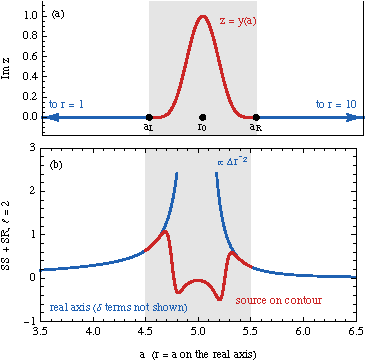
\includegraphics[width=\columnwidth]{prl_intro.pdf}
\caption{(a) The contour $z=y(a)$ in the complex $r$ plane (red). Outside the worldtube (shaded) the radial coordinate stays on the real axis (blue).
(b) The $\ell=2$ second-order source of the model below, with an exact puncture. On the real axis (blue) $\mathrm{SS}+\mathrm{SR}$ diverges as $\Delta r^{-2}$ at $r_0$; the $\delta$ terms of SR are not shown. On the contour (red) the real part of the continued source $\tilde s(y(a))$ is bounded and joins the real-axis source at the worldtube boundaries. Its imaginary part, the shadow, is shown in Fig.~\ref{fig:source}(b).}
\label{fig:intro}
\end{figure}

%=====================================================================
\emph{Model.}---%
We consider a scalar charge $q$ at $\x_0=r_0\hat{\bm z}$ in flat space:
\begin{equation}
\nabla^2\Phi_1=-4\pi q\,\delta^3(\x-\x_0),
\qquad
\nabla^2\Phi_2=\tfrac12\partial_z^2\big(\Phi_1^2\big).
\label{eq:model}
\end{equation}
We split $\Phi_1=\PhiS+\PhiR$, with $\PhiS=q/\rho$, $\rho=|\x-\x_0|$, and a regular field $\PhiR=c_0+c_1z$ injected through the boundary conditions.
With $Q[A,B]:=\tfrac12\partial_z^2(AB)$, the source splits as $Q[\Phi_1,\Phi_1]=\mathrm{SS}+2\,\mathrm{SR}+\mathrm{RR}$.

The source is a second derivative of the locally integrable $\Phi_1^2$, so it is a well-defined distribution.
Pointwise, $\mathrm{SS}\sim\rho^{-4}$ and $\mathrm{SR}\ni q\PhiR\,\partial_z^2\rho^{-1}\sim\rho^{-3}$.
This mirrors the gravitational case, where $\delta^2G$ is defined through linear operators acting on integrable functions~\cite{MusaeusPoundUpton2026}.
Because $\partial_z$ commutes with $\nabla^2$, the exact solution is $\Phi_2=\tfrac12\partial_z^2\chi$, where $\nabla^2\chi=\Phi_1^2$ is solved in closed form.

We decompose into axisymmetric modes, $\Phi=\sum_\ell\phi_\ell(r)Y_{\ell0}(\theta)$, so that $[\nabla^2\Phi]_\ell=\Lop\phi_\ell$ with $\Lop=\partial_r^2+\tfrac2r\partial_r-\tfrac{\ell(\ell+1)}{r^2}$.
Near $r_0$, with $\Delta r=r-r_0$, the SS modes behave as $A_\ell/\Delta r^2+B_\ell/\Delta r+C_\ell\ln|\Delta r|$.
The SR modes contain jumps and a term $c_\ell\,\delta(\Delta r)$, with $c_\ell=-4\pi q\PhiR(\x_0)Y_{\ell0}(0)/r_0^2$.
Figure~\ref{fig:source}(a) shows both for $\ell=2$.

%=====================================================================
\emph{Contour.}---%
Inside a worldtube $[a_L,a_R]=[r_0-R,r_0+R]$ we replace $r$ by $z=y(a)=a+i\eta\big[1-(a-r_0)^2/R^2\big]^6$, which lies in the upper half-plane.
Outside the worldtube $z$ stays real.
The first-order point source becomes $\dext(z)$, whose boundary value is $\dext(r+i0)=\delta(\Delta r)+\tfrac{i}{\pi}\mathrm{P}\tfrac{1}{\Delta r}$.
The physical source is its real part; the imaginary part is the ``shadow''.

The method rests on one elementary property of the linear solves.
Let $\tilde s$ be analytic above the real axis inside the worldtube, with $\Re\tilde s(r+i0)=s$, and integrate $\Lop\tilde\psi=\tilde s$ along the contour from real data at $a_L$.
Then $\Re\tilde\psi(r+i0)$ solves $\Lop\psi=s$, and $\Re\tilde\psi$ and $\Re\tilde\psi'$ at $a_R$ are the physical exterior data.
This holds because $\Lop$ has real coefficients that are analytic near $r_0$.
Since $\Re(\Delta r+i0)^{-n}$ is the Hadamard finite part of $\Delta r^{-n}$~\cite{GelfandShilov}, the contour performs mode-level Hadamard regularization automatically.
It also turns derivatives of kinks into $\dext$ poles, so the $\delta$ content of the source is generated without any book-keeping.

Two consistency conditions make the singular/regular split on the contour match the split in 3D.
(i) The real part of each continued singular mode must be the $\ell$-mode of the \emph{same} 3D puncture $\PhiP$ used in SS and SR.
(ii) $\dext-\Lop\phi^{\rm P}_\ell$ must be real on the axis.
Condition (i) excludes, for example, the convenient particular solution of the mode equation with integration constants set to zero.
With real-coefficient antiderivatives, its real part is a one-sided Green's function. It differs from the Coulomb mode by a homogeneous solution, and in 3D it removes $q/\rho$ entirely outside $r=r_0$.
Condition (ii) prevents a spurious shadow in the residual field.
Condition (i) is the same requirement as in real-axis puncture schemes~\cite{Upton2026}; condition (ii) has no real-axis analogue.
Both are discussed in Appendix~\ref{app:consistency}.

%=====================================================================
\begin{figure*}[t]
\centering
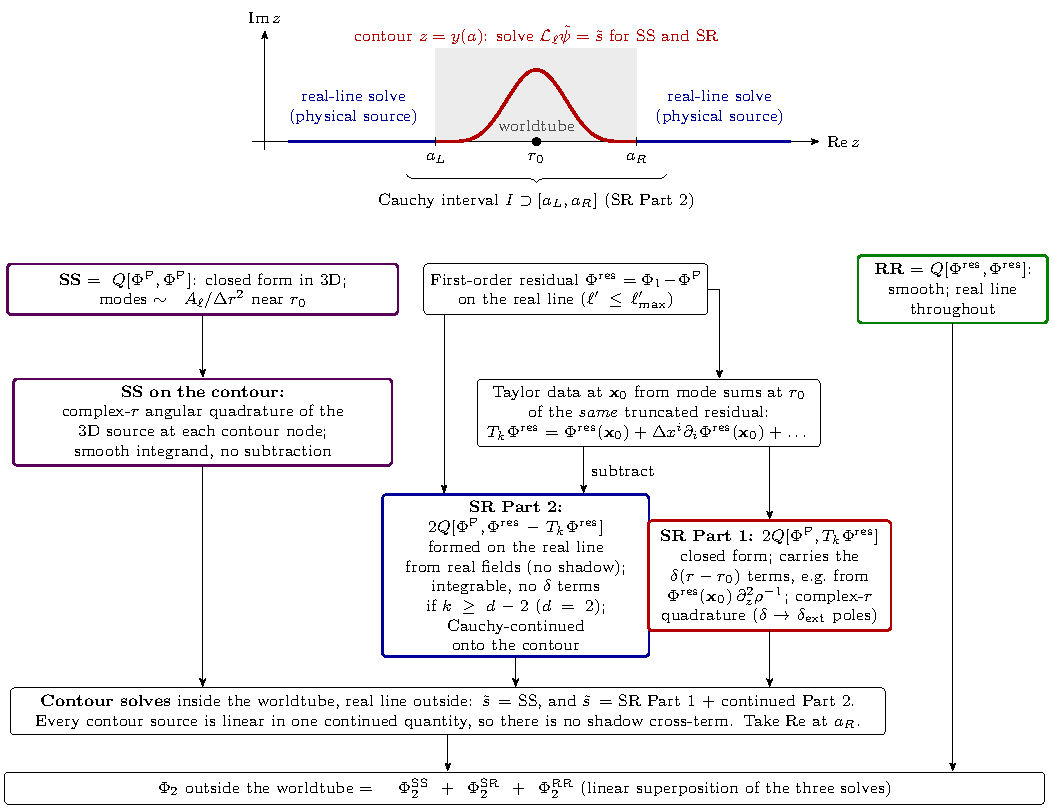
\includegraphics[width=\textwidth]{fig_flowchart.pdf}
\caption{The second-order pipeline.
\emph{Top:} the complex $r$ plane. SS and SR are solved on the contour inside the worldtube and on the real axis, with the physical source, outside it.
\emph{Bottom:} the treatment of each piece.
SS is evaluated directly on the contour by angular quadrature at complex $r$ (Appendix~\ref{app:quadrature}).
SR is split into a closed-form Part 1, which carries all non-integrable and $\delta$ terms, and an integrable Part 2, which is formed on the real axis from real fields and either solved there or Cauchy-continued onto the contour and solved with Part 1 (dashed arrows).
RR is smooth and solved on the real axis.}
\label{fig:flow}
\end{figure*}

\emph{Nonlinearity and the hybrid split.}---%
If two continued fields $u_j+iv_j$ are multiplied on the contour, the real part of the product contains $-v_1v_2$.
The shadow then contaminates the real (physical) second-order field.
We therefore require every contour source to be linear in a single continued quantity (Fig.~\ref{fig:flow}).

\emph{SS} is built from the closed-form 3D expression $Q[\PhiP,\PhiP]$, never from products of modes (as including the full singular field would require an infinite sum of modes).
At fixed angle $\theta\neq0$ that expression is analytic in $r$ near $r_0$; its singularity lies at complex radius $r_0e^{\pm i\theta}$.
So we evaluate the SS modes directly on the contour by angular quadrature at complex $r$.
Using a complex $r$ allows the integrand to be smooth.
The only subtlety is the point where the contour crosses $|z|=r_0$, where the singular angle reaches the real $\theta$ axis.
Integrating over $\rho$ instead of $\cos\theta$ makes the integrand a Laurent polynomial with its only singularity fixed at $\rho=0$; a path that keeps $\rho=0$ on one side then gives the continuation, including where the contour crosses $|z|=r_0$ (Appendix~\ref{app:quadrature}).

\emph{SR} involves the residual field $\Pres=\Phi_1-\PhiP$, which is known only through its modes on the real axis.
With a truncated puncture, the continued residual modes carry a shadow, and the cross term grows like $(1+R/r_0)^{\ell'}$ with the coupled mode number $\ell'$ (Appendix~\ref{app:shadow}).
We therefore split SR using the Taylor polynomial $T_k\Pres$ of the residual about $\x_0$, of order $k$:
\begin{equation}
2Q[\PhiP,\Pres]=\underbrace{2Q[\PhiP,T_k\Pres]}_{\rm Part\ 1}+\underbrace{2Q[\PhiP,\Pres-T_k\Pres]}_{\rm Part\ 2}.
\label{eq:hybrid}
\end{equation}
Part 1 is closed form; we can therefore extend it to the complex plane. It carries every non-integrable and $\delta$ term, for example the $\delta$ from $\Pres(\x_0)\partial_z^2\rho^{-1}$, and is evaluated by complex-$r$ quadrature.
For pieces with kinks at $r_0$, the inside and outside branches are blended with $H(z)=1+\tfrac{i}{\pi}\ln(z-r_0)$ before $\partial_z^2$ is applied, so the $\delta$ terms become $\dext$ poles.
Part 2 contains $\Pres-T_k\Pres=O(\rho^{k+1})$, which vanishes on the worldline even though $\Pres$ does not.
When $Q$ puts $d$ derivatives on $\PhiP$, Part 2 is $O(\rho^{k-d})$; for $k\ge d-2$ it is integrable and has no $\delta$ terms.
Here $d=2$, so $k=0$ suffices.
Part 2 is therefore formed on the real axis, where both factors are real, and continued with
\begin{equation}
\tilde s(z)=\int_I s(t)\,\dext(z-t)\,dt=\frac{1}{\pi i}\int_I\frac{s(t)}{t-z}\,dt
\label{eq:cauchy}
\end{equation}
over an interval $I$ slightly larger than the worldtube. This is analytic above the axis and has $\Re\tilde s(r+i0)=s$.
Being integrable and free of $\delta$ terms, Part 2 can be solved on the real axis like RR, with the solve split at $r_0$; nothing is subtracted, so nothing is amplified.
Alternatively, it can be continued onto the contour with Eq.~\eqref{eq:cauchy} and solved together with Part 1, which is what our tests did; the two routes agree to $2\times10^{-16}$ (Appendix~\ref{app:convergence}).
The continuation is a fixed linear map from real-axis samples to contour nodes, independent of $\ell$, so it is cheap, but it is not necessary: only Part 1 needs the contour.
$T_k$ is computed from the same truncated mode sums of $\Pres$ at $r_0$ as enter Part 2.
The two parts then add up exactly to the truncated SR, so errors in the local data are absorbed into the ordinary mode truncation.

\emph{RR} is smooth and is solved on the real axis throughout.
The exterior field is the sum of the three linear solves.

%=====================================================================
\begin{figure*}[t]
\centering
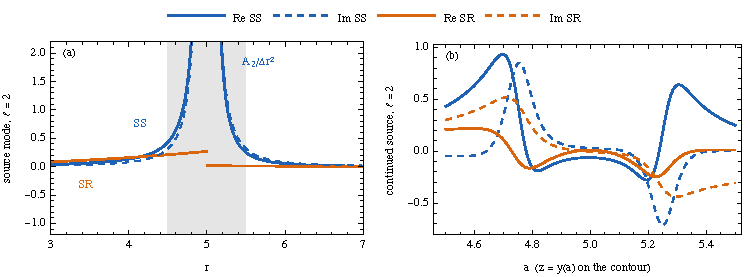
\includegraphics[width=\textwidth]{prl_source.pdf}
\caption{The $\ell=2$ source modes for $q=1$, $r_0=5$, $\PhiR=1+z/10$.
(a) On the real axis. SS diverges as $A_2/\Delta r^2$. SR is bounded, with a jump at $r_0$, and also contains a $\delta(\Delta r)$ term with coefficient $c_2=-0.476$ (not shown). The worldtube is shaded.
(b) On the contour $z=y(a)$, with real parts solid and imaginary parts dashed. Both sources are smooth there.}
\label{fig:source}
\end{figure*}

\emph{Results with an exact puncture.}---%
We take $q=1$, $r_0=5$, $R=\tfrac12$, $\eta=1$ and $c_0=1$, $c_1=\tfrac1{10}$, and working precision 30.
All radial solves use the physical boundary conditions $\psi'=\ell\psi/r$ at $r=1$ and $\psi'=-(\ell+1)\psi/r$ at $r=10$, which select the solutions regular at $r=0$ and decaying at infinity.
With $\PhiP=\PhiS$, the residual is $\PhiR$ and SR needs only $\ell'\in\{0,1\}$.
Figure~\ref{fig:source}(b) shows the continued sources.
The recovered exterior modes agree with the exact solution to below $3\times10^{-18}$ for $\ell\le6$ (Fig.~\ref{fig:solution}).
Fitting the SS and SR errors to point-supported terms (modes of $q/\rho$ and $\partial_{r_0}q/\rho$) gives coefficients below $1.1\times10^{-18}$, so the contour selects the canonical distributional source with no extra worldline terms.
Complex-$r$ quadrature of SS agrees with the closed-form continuation to $2\times10^{-14}$ on the contour, at a cost comparable to real-axis quadrature near $r_0$.
It also needs about as many radial source samples as real-axis finite-part integration, but nothing singular is subtracted, so errors in the samples are not amplified: with $10^{-8}$ relative noise, the exterior field is $10^2$--$3\times10^5$ times more accurate than on the real axis (Appendix~\ref{app:cost}).
By contrast, discarding the $\delta(\Delta r)$ terms, as a pointwise real-axis treatment of SR would, gives errors of $0.55$ to $3.3$.

\begin{figure}[t]
\centering
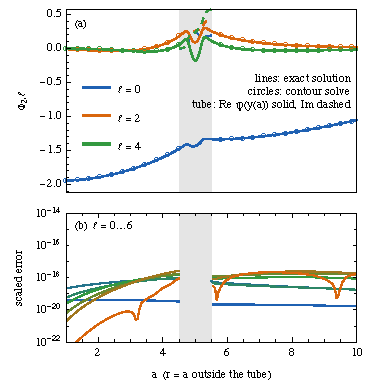
\includegraphics[width=\columnwidth]{prl_solution.pdf}
\caption{(a) Recovered exterior modes $\Phi_{2,\ell}$ (circles) against the exact solution (lines), for an exact puncture, plotted against $a$ ($r=a$ outside the worldtube).
Both satisfy the physical boundary conditions; the exact solution is $\tfrac12\partial_z^2\chi$ plus the homogeneous terms $r^\ell$ and $r^{-\ell-1}$ that meet them.
Inside the worldtube the curves show the real (solid) and imaginary (dashed) parts of the contour solution $\tilde\psi_\ell(y(a))$; these are not physical values of $\Phi_2$.
(b) Error scaled by $\max_r|\Phi_{2,\ell}|$, for $\ell=0$--$6$, outside the worldtube.}
\label{fig:solution}
\end{figure}

\emph{Results with truncated punctures.}---%
To mimic the self-force situation we use a puncture defined in 3D, $\PhiP=q/\rho+cq\rho^n$, with $n$ odd and $c=r_0^{-(n+1)}$, consistently in every piece.
The residual $\PhiR-cq\rho^n$ is then only $C^{n-1}$ at $\x_0$, and has modes at every $\ell'$.
Figure~\ref{fig:convergence} compares three treatments of SR.
Multiplying continued modes gives an error that first follows the mode truncation, then grows once the shadow cross-term takes over, near $\ell'_{\max}=12$--$16$.
Cauchy-continuing the whole real-axis SR fails with an error of order one, because it misses the $\delta$ terms.
The hybrid split~\eqref{eq:hybrid} coincides with the mode-truncation error at every $\ell'_{\max}$, for every $k=0$--$3$.
That error converges as $\ell'^{-(n+2)}_{\max}$, with fitted slopes $2.93$, $4.87$, $6.83$ and $8.79$ for $n=1$, 3, 5 and 7.
Fitting the large-$\ell'$ tail with the functions of Refs.~\cite{Upton2026,HeffernanOttewillWardell2012} gains a factor of 18--40 at $\ell'_{\max}=20$ (Appendix~\ref{app:convergence}).
The remaining error is the same algebraic mode-coupling convergence that real-axis puncture schemes encounter~\cite{Upton2026}. The contour adds nothing to it.

\begin{figure}[t]
\centering
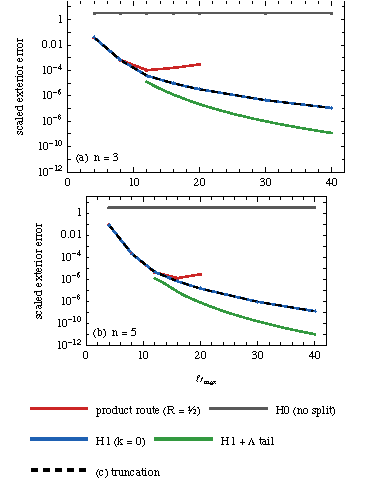
\includegraphics[width=\columnwidth]{prl_convergence.pdf}
\caption{Scaled exterior error against $\ell'_{\max}$ for the truncated puncture $q/\rho+cq\rho^n$, with (a) $n=3$ and (b) $n=5$, and $R=\tfrac12$.
Red: product of continued modes. Grey: Cauchy continuation of the whole SR (no split). Blue: hybrid split ($k=0$). Black dashed: mode-truncation error alone. Green: hybrid with large-$\ell'$ tail fitting.}
\label{fig:convergence}
\end{figure}

%=====================================================================
\emph{Relation to recent work.}---%
\emph{Musaeus, Pound and Upton (MPU)}~\cite{MusaeusPoundUpton2026} write the canonical second-order source as $\mathrm{Pf}\,\delta^2G+8\pi T_Q$.
Here $T_Q$ is a $\delta$ function on the worldline, linear in the regular field.
They show that SR modes contain only jumps and $\delta$ terms and their derivatives, as in our model.
On their flat-space Teukolsky example, with sources up to $\Delta r^{-4}$, the contour reproduces their mode-level finite part (their Eqs.~141 and A2--A5) to $4\times10^{-34}$ for $\ell=2$--$6$, and confirms their closed form for $\ell=2$.
In our model, $T_Q=-\tfrac{4\pi}{3}q\PhiR(\x_0)\delta^3(\x-\x_0)$, and the mode-level $\delta$ coefficient $c_\ell$ splits as $\tfrac23c_\ell$ from the 4D finite part (a ball-excluded principal value) plus $\tfrac13c_\ell$ from $T_Q$.
Their Eq.~24 is exact when the modes are those of the 4D finite-part distribution.
Applied to pointwise mode functions, however, the mode-level reduction (their Eq.~105) misses the $\tfrac23c_\ell$, because the ball and shell regulators do not commute for the trace-free $\rho^{-3}$ term.
Conversely, when source modes are built by coupling kinked mode functions with distributional derivatives, as in practice~\cite{Upton2026}, $T_Q$ is already included, and adding it again would double-count it.
The contour, applied to operators acting on continued integrable functions, yields the canonical source directly, with no separate $T_Q$.

\emph{Upton et al.}~\cite{Upton2026} enforce the same consistency conditions as ours in production: the same puncture and residual in every piece, and an exact puncture mode decomposition rather than a series in $\Delta r$.
Their dominant costs are the SS quadrature near the worldline and the construction of $h^{\rm P2}$.
The contour approach needs no $h^{\rm P2}$.
Further, our complex-$r$ quadrature replaces near-singular real-axis integrals with smooth ones.
An alternative for SS (Appendix~\ref{app:ssroutes}) subtracts the singular terms of the local expansion in $\Delta r$ from real-axis data and Cauchy-continues the rest; it is equivalent in content to MPU's Hadamard subtraction.
It amplifies quadrature noise by $3\times10^2$--$4\times10^3$ near $r_0$, which is why we prefer complex-$r$ quadrature.
In the toy, the largest saving in SS quadrature comes from evaluating the source once per point and projecting it onto all modes, a factor of 200--2000 over adaptive quadrature for each mode; this applies on the real axis as well (Appendix~\ref{app:cost}).

%=====================================================================
\emph{Conclusion.}---%
Continuing each mode equation onto a contour around the particle gives automatic, puncture-free regularization of second-order point-particle sources.
It reproduces the Hadamard finite part and the $\delta$ content of the canonical distributional source.
The nonlinear difficulty, contamination by the shadow, is removed by keeping every contour source linear in a single continued quantity: closed-form singular pieces are evaluated at complex radius, regular-field remainders are formed on the real axis, where they can be solved directly or continued by a Cauchy integral, and the smooth RR piece stays on the real axis.
In a scalar model with the $1/\rho^4$ distributional structure of gravity, the method is accurate to $10^{-17}$ with exact punctures.
With truncated punctures it converges at the rate set by the residual's smoothness, adding no error beyond the usual mode truncation.
Next steps are the Lorenz-gauge and Teukolsky sources in Schwarzschild.
There, complex-$r$ quadrature of $\delta^2R[h^{\rm P1},h^{\rm P1}]$ avoids subtracting singular terms from numerically integrated source samples, and the toy suggests that sharing source evaluations across modes, on either axis, could reduce the dominant cost of current calculations.

\begin{acknowledgments}
% TODO: acknowledgments and funding.
\end{acknowledgments}

%=====================================================================
\appendix
\setcounter{secnumdepth}{1}

\section{Conventions and the linear-solve property}\label{app:conventions}
Modes are $\Phi=\sum_\ell\phi_\ell(r)Y_{\ell0}(\theta)$, with $[f]_\ell=\sqrt{\pi(2\ell+1)}\int_{-1}^1 f\,P_\ell(\mu)\,d\mu$ and $\mu=\cos\theta$.
The first-order mode source is $\kappa_\ell\,\delta(r-r_0)$, with $\kappa_\ell=-(q/r_0^2)\sqrt{4\pi(2\ell+1)}$.
The Coulomb mode for $\kappa_\ell=1$ is $G_\ell=-r_0^2\,r_<^\ell/[(2\ell+1)r_>^{\ell+1}]$.

We use $H(z)=1+\tfrac{i}{\pi}\log(z-r_0)$ with the principal logarithm, and real-axis values are boundary values from above.
Logarithms of the form $\log[c(z-z_*)]$ are rewritten as $\ln|c|+\log(z-z_*)-i\pi[c<0]$.
This is the same function in the upper half-plane, and its principal value on the axis is the value from above.
Without this rewrite, Mathematica's $\log(r_0-r)$ at real $r>r_0$ lies on the wrong side of the cut.

\emph{Linear-solve property.}
$\Lop$ has real coefficients that are analytic away from $z=0$.
The solution continued along the contour therefore equals the boundary value from above of the solution in the region between the contour and the real segment.
Taking real parts commutes with $\Lop$, so $\Re\tilde\psi(r+i0)$ solves $\Lop\psi=\Re\tilde s(r+i0)$ with the same real data at $a_L$.
Because $(\Delta r+i0)^{-n}=\mathrm{FP}\,\Delta r^{-n}+i\pi(-1)^n\delta^{(n-1)}(\Delta r)/(n-1)!$, the real part is the Hadamard finite part.

\section{Consistency of the continued singular mode}\label{app:consistency}
\emph{(i) Real part.}
Any solution $\psi$ of $\Lop\psi=\dext$ satisfies $\Re\psi(r+i0)-G_\ell=\alpha r^\ell+\beta r^{-\ell-1}$, because both sides solve the same real equation with the same $\delta$ source.
The singular structure at $r_0$ does not fix $\alpha$ and $\beta$; the 3D puncture does.

\texttt{DSolve}'s particular solution with constants set to zero gives the following ($\ell\le12$ checked):
\begin{itemize}
\item $\ell=0$: an anti-physical Green's function, $(\alpha,\beta)=(r_0,r_0^2)$;
\item $\ell=1$: the Coulomb mode;
\item $\ell\ge2$: a one-sided Green's function that vanishes for $r<r_0$, $\alpha=r_0^{1-\ell}/(2\ell+1)$.
\end{itemize}
Summed in 3D, these offsets give $\Delta=-q/\rho+q\,r\cos\theta/r_0^2-q/r$ for $r<r_0$, and diverge for $r>r_0$.
If such a mode is used with 3D SS and SR, the computed second-order source is $Q[\Phi_1-\Delta,\Phi_1-\Delta]$ instead of $Q[\Phi_1,\Phi_1]$.

\emph{(ii) Imaginary part.}
Replacing $\Theta\to H$ in the Coulomb mode does not give a solution of $\Lop\psi=\dext$, because $\dext$ is not annihilated by smooth factors that vanish at $r_0$.
For $\ell=0$, $\mathcal L_0[-r_0+(r_0-r_0^2/z)H]=\dext-\tfrac{i}{\pi}z^{-1}$, and the residual field acquires an $O(1)$ shadow, $r/(2\pi)$.
The fix is to add $\tfrac{i}{2\pi}z$.
Equivalently, use $\psi_p-D_\ell$, where $D_\ell$ is the homogeneous offset found in (i).

\section{Complex-\texorpdfstring{$r$}{r} angular quadrature, step by step}\label{app:quadrature}
We take the SS source of the model as the example:
\begin{equation}
S(r,\mu)=\tfrac12q^2\,\partial_z^2\rho^{-2}=\tfrac12q^2\big(-2\rho^{-4}+8d^2\rho^{-6}\big),
\end{equation}
where $\rho^2=r^2+r_0^2-2rr_0\mu$ and $d=r\mu-r_0$ is the $z$-component of $\x-\x_0$.
Its modes are
\begin{equation}
\mathrm{SS}_\ell(r)=\sqrt{\pi(2\ell+1)}\int_{-1}^{1}S(r,\mu)\,P_\ell(\mu)\,d\mu.
\label{eq:SSmode}
\end{equation}
The aim is to evaluate this at the contour nodes $r\to z=y(a)$.

\emph{Step 1: where the difficulty comes from.}
At complex $z$ the integrand is singular where $\rho^2=0$, i.e.\ at
\begin{equation}
\mu^*(z)=\frac{z^2+r_0^2}{2zr_0}=\frac12\Big(\frac{z}{r_0}+\frac{r_0}{z}\Big).
\end{equation}
Writing $z=|z|e^{i\varphi}$ gives $\Im\mu^*=\tfrac12\sin\varphi\,(|z|/r_0-r_0/|z|)$.
So $\mu^*$ is real, and lies in $[-1,1]$, exactly when $|z|=r_0$.
Every contour from $a_L<r_0$ to $a_R>r_0$ crosses the circle $|z|=r_0$, at some point $z_c=r_0e^{i\varphi_c}$, where $\mu^*=\cos\varphi_c$ lies on the integration segment.
On either side of $z_c$, $\mu^*$ is on opposite sides of the real $\mu$ axis.
On our contour, $\mu^*$ starts just beyond $\mu=1$ at $a_L$, passes below the segment, through it at $z_c$ and above it, and ends just beyond $\mu=1$ at $a_R$ (Fig.~\ref{fig:quad}a,b).
Integrating along the straight segment $\mu\in[-1,1]$ would therefore jump by $2\pi i$ times a residue as $z$ passes $z_c$, and would not give an analytic function of $z$.
Before $z_c$ the straight segment gives the continuation from $a_L$; after $z_c$ it gives the continuation from $a_R$.
A $\mu$ contour that stays on one branch must keep $\mu^*(z)$ on the same side for every $z$.
For the continuation from $a_L$ it must detour above $\mu^*(z_c)$ at the crossing (violet curve in Fig.~\ref{fig:quad}b), and keep passing above $\mu^*(z)$ afterwards, even where $\mu^*(z)$ has left the axis and the straight segment no longer touches it.
Its shape depends on $z$, so constructing it means following $\mu^*(z)$ along the whole $r$ contour.

\begin{figure*}[t]
\centering
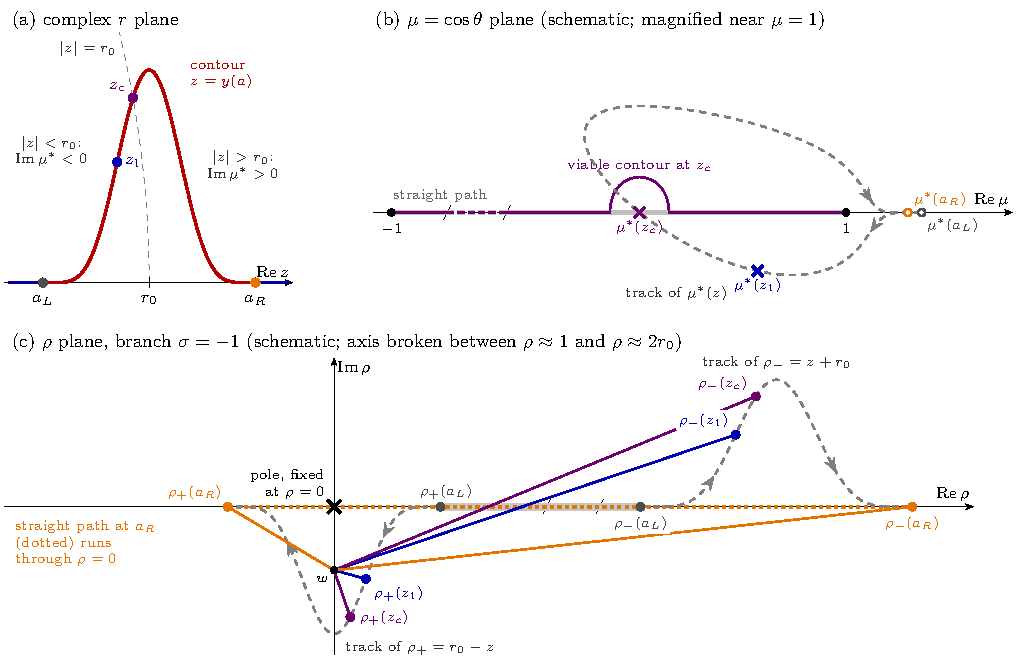
\includegraphics[width=\textwidth]{fig_quadrature.pdf}
\caption{Why the angular integral is done in $\rho$.
Colours mark the points $z_1$, $z_c$ and $a_R$ of the contour in (a), and grey marks $a_L$.
(a)~The contour $z=y(a)$ crosses the circle $|z|=r_0$ at $z_c$.
(b)~The $\mu$ integral runs from $-1$ to $1$; the axis is broken, and the region near $\mu=1$ is magnified.
The dashed curve is the singular angle $\mu^*(z)$ as $z$ runs along the contour.
At real $r$ it lies on the real axis beyond $\mu=1$, outside the integration range (open circles, $z=a_L$ and $a_R$).
Along the contour it passes below the straight path (at $z_1$), through it (at $z_c$) and then above it, so the straight-path integral jumps at $z_c$.
A viable contour must keep $\mu^*(z)$ on the side it started on.
For the branch continued from $a_L$ it must detour above $\mu^*(z_c)$, as shown in violet, and keep passing above $\mu^*(z)$ for every later $z$, even though the straight path no longer touches $\mu^*(z)$ there.
Finding this contour is not straightforward: its shape changes with $z$, and it can only be fixed by following $\mu^*(z)$ along the whole $r$ contour.
(c)~In $\rho$ the pole stays at $\rho=0$; only the endpoints $\rho_-=z+r_0$ and $\rho_+=r_0-z$ move.
The dashed tracks show where they go as $z$ runs from $a_L$ to $a_R$ (arrows), starting from $\rho_\pm(a_L)$ (grey), which are joined by the physical path at $a_L$ (thick grey segment on the real axis).
Each coloured path runs $\rho_-(z)\to w=-i/2\to\rho_+(z)$, the same recipe for every $z$, and never touches the pole.
At $a_R$, $\rho_+=-R$ lies on the real axis on the far side of the pole, and the straight path from $\rho_-$ to $\rho_+$ (orange dotted) runs through it.
The branch $\sigma=+1$ is the mirror image in the upper half-plane.}
\label{fig:quad}
\end{figure*}

\emph{Step 2: change variable from $\mu$ to $\rho$.}
Use the distance from the particle as the integration variable.
From $\rho^2=z^2+r_0^2-2zr_0\mu$:
\begin{gather}
\mu(\rho)=\frac{z^2+r_0^2-\rho^2}{2zr_0},\qquad
d\mu=-\frac{\rho\,d\rho}{zr_0},\nonumber\\
d(\rho)=z\mu-r_0=\frac{z^2-r_0^2-\rho^2}{2r_0}.
\end{gather}
Both $\mu$ and $d$ are polynomials in $\rho^2$, so $P_\ell(\mu(\rho))$ is too, and
\begin{gather}
\mathrm{SS}_\ell(z)=\sqrt{\pi(2\ell+1)}\int_{\rho_-}^{\rho_+}f_\ell(\rho;z)\,d\rho,\nonumber\\
f_\ell=-\frac{\rho}{zr_0}\,S\,P_\ell\big(\mu(\rho)\big).
\label{eq:rhoint}
\end{gather}
The integrand $f_\ell$ is a Laurent polynomial in $\rho$, with powers down to $\rho^{-5}$.
Its only singularity is a pole at $\rho=0$, and this stays \emph{fixed} as $z$ moves along the contour.
Because $S$ and $P_\ell(\mu(\rho))$ depend only on $\rho^2$, $f_\ell$ is odd in $\rho$.

\emph{Step 3: the endpoints.}
$\mu=-1$ maps to $\rho_-=z+r_0$, and $\mu=+1$ maps to $\rho_+=\sigma(z-r_0)$ with $\sigma=\pm1$.
On our contour, $\Re\rho_-\approx2r_0$ and $|\rho_+|=|z-r_0|\ge0.29$, so neither endpoint comes near the pole.
The endpoints move with $z$; the singularity does not.

\emph{Step 4: the path.}
Integrate along two straight segments, $\rho_-\to w\to\rho_+$, with waypoint $w=\sigma i/2$.
For $\sigma=+1$, both $w$ and $\rho_+=z-r_0$ lie in the closed upper half-plane; for $\sigma=-1$, both lie in the closed lower half-plane.
In either case the second segment never meets $\rho=0$, and the first passes at a distance of about $\tfrac12$ from it.
As $z$ moves along the contour, including through $z_c$, the endpoints move continuously and the path never sweeps across $\rho=0$.
By Cauchy's theorem the integral~\eqref{eq:rhoint} is therefore an analytic function of $z$ along the whole contour (Fig.~\ref{fig:quad}c).
Mapped back to the $\mu$ plane, the path is a curve from $-1$ to $1$ that keeps $\mu^*(z)$ on the same side for every $z$, the side being fixed by $\sigma$, like the violet curve in Fig.~\ref{fig:quad}b.
No special treatment is needed at the crossing.
The waypoint matters near the ends of the contour.
A straight path from $\rho_-$ to $\rho_+=r_0-z$ also misses the pole for $z$ in the upper half-plane, but it comes within $0.002$ of it for $a\ge5.4$, and at $a_R$, where $\rho_+=-R$ is real, it runs through it (orange dotted in Fig.~\ref{fig:quad}c).
The path via $w$ can also be deformed, without crossing $\rho=0$, onto a route along the grey tracks in Fig.~\ref{fig:quad}c: back along the track of $\rho_-$ to $\rho_-(a_L)$, along the physical path to $\rho_+(a_L)$, then along the track of $\rho_+$ to $\rho_+(z)$.
That route is the physical path at $a_L$ dragged continuously to $z$, which shows directly that the integral is the continuation from $a_L$.
It would serve equally well as the integration path, but it has three pieces, two of them curved, whose lengths depend on the contour between $a_L$ and $z$; the path via $w$ has two straight pieces and depends only on the current $z$.
Two contours are therefore involved: the $r$ contour, on which the source is needed, and, for each node $z$ on it, a path in $\rho$ for the angular integral.

\emph{Step 5: the two branches.}
Since $f_\ell$ is odd, its antiderivative is even in $\rho$, except for the term $a_{-1}\log\rho$ that comes from the $\rho^{-1}$ term $a_{-1}(z)/\rho$ of $f_\ell$.
The endpoints $\rho_+=\pm(z-r_0)$ therefore give results that differ only through this logarithm, by $\pm i\pi a_{-1}(z)$.
In the $\mu$ plane this is $2\pi i$ times the residue at $\mu^*$: the two branches pass $\mu^*$ on opposite sides.
The same term produces the $\log(z-r_0)$ in the mode function.
\begin{itemize}
\item For real $r<r_0$, the physical path runs along the positive real $\rho$ axis from $r_0+r$ to $r_0-r$, which is the $\sigma=-1$ endpoint. So $\sigma=-1$ continues the inside expression, from $a_L$.
\item For $r>r_0$, the physical endpoint is $r-r_0$, so $\sigma=+1$ continues the outside expression, from $a_R$.
\end{itemize}
For real $z$, $a_{-1}$ is real, so the two branches differ by a quantity that is imaginary on the axis.
For SS, therefore, either branch has the correct real part and can be used.
The $\sigma=+1$ branch agrees with the closed-form continuation of $\mathrm{SS}_\ell$ to $1.8\times10^{-14}$ on the contour.
The $\sigma=-1$ branch differs from it there by 2--30\%, but by a function that is imaginary on the axis, and it gives the exterior field to $2\times10^{-14}$.

\emph{Step 6: pieces with kinks.}
For SR Part 1 the mode functions have kinks at $r_0$, inherited from the Coulomb modes $r_<^L/r_>^{L+1}$.
The inside and outside branches then differ by a real-analytic function, not just by an imaginary term, and neither alone has the correct real part on both sides.
We therefore evaluate both branches of the \emph{undifferentiated} product modes $F_j=[2\PhiP T_k\Pres]_j$, together with their $r$-derivatives at fixed $\mu$, and blend them:
With the jump $J=F_{\rm out}-F_{\rm in}$,
\begin{align}
\tilde F&=F_{\rm in}+JH,\qquad
\tilde F'=F'_{\rm in}+J'H+JH',\nonumber\\
\tilde F''&=F''_{\rm in}+J''H+2J'H'+JH''.
\end{align}
Only then is the $\partial_z^2$ ladder applied in mode space.
The terms with $H'=\dext$ and $H''=\dext'$ carry the $\delta$ content of SR.
This gives the full SR (exact puncture) to $4\times10^{-14}$ and Part 1 to $1.1\times10^{-13}$.
The inside branch alone is wrong by factors of 4 to 1200.
Blending the finished, differentiated source instead loses the $H'$ and $H''$ terms, with errors of 3 to 900.

\emph{Step 7: numerics and cost.}
Each segment uses 80-node Gauss--Legendre quadrature at working precision 30, so each contour node costs 160 evaluations of the 3D source; 64 nodes per segment suffice for $10^{-8}$.
The integrand is a smooth function of $\rho$ on both segments, so no adaptive refinement is needed, and the result is accurate to $10^{-14}$.
The nodes do not depend on $\ell$, so the source can be evaluated once per node and projected onto all modes with the Legendre recurrence.
On the real axis, a fixed rule in $\ln\rho$ does as well per point (56--80 nodes), while adaptive quadrature for each $(\ell,r)$ separately takes 450--3500 evaluations.
The costs are compared in Appendix~\ref{app:cost}.

\emph{Step 8: towards GR.}
In the rotated coordinates $(\alpha,\beta)$ used for Schwarzschild punctures~\cite{Upton2026}, the leading distance at fixed $\beta$ has the form $\rho_0^2=(\Delta r\text{ term})+\chi(\beta)(1-\cos\alpha)$, which is linear in $\cos\alpha$.
Substituting $\rho_0$ for $\alpha$ at fixed $\beta$ should again turn a puncture built from powers of $\rho_0$ and polynomials, including polynomial window functions, into a Laurent polynomial with a fixed pole at $\rho_0=0$.
Terms in $\ln\rho_0$, from higher-order punctures, introduce a branch point instead of a pole. A fixed path with the cut placed away from it should still work.
This extension is untested.

\section{Shadow growth with truncated punctures}\label{app:shadow}
With $\PhiP=q/\rho+cq\rho^n$ used consistently, the real-part mismatch vanishes identically.
The remaining contamination from products of continued modes is linear in $c$.
At fixed $\ell'_{\max}$ it falls by about $0.07$--$0.08$ per unit of $n$, but each coupled mode's contribution grows with $\ell'$.
Near $\ell'=30$ the growth per mode is $1.12$ and $1.19$ for $R=\tfrac12$, and $1.06$ and $1.09$ for $R=\tfrac14$, for the $Q=AB$ and $Q=\nabla A\cdot\nabla B$ toys respectively.
These are close to $1+R/r_0$ times a slowly varying power.

For fixed $R$ the total error therefore has a minimum in $\ell'_{\max}$.
Shrinking the worldtube as modes are added, $R=r_0/\ell'_{\max}$, keeps $(1+R/r_0)^{\ell'_{\max}}$ bounded, and the error then falls monotonically (Fig.~\ref{fig:lprime}).
For $Q=\tfrac12\partial_z^2(AB)$ the minimum lies near $\ell'_{\max}=12$--$16$ (Fig.~\ref{fig:convergence}).
The hybrid split removes the contamination entirely.

\begin{figure*}[t]
\centering
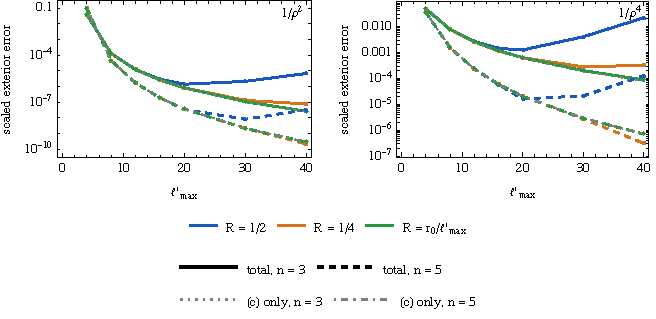
\includegraphics[width=0.75\textwidth]{fig_lprime_optimum.pdf}
\caption{Products of continued modes with a truncated puncture, for $Q=AB$ (left) and $Q=\nabla A\cdot\nabla B$ (right).
Exterior error against $\ell'_{\max}$ for $n=3$ (solid) and $n=5$ (dashed): fixed worldtubes $R=\tfrac12,\tfrac14$, and a shrinking worldtube $R=r_0/\ell'_{\max}$.
Dotted: mode-truncation error.}
\label{fig:lprime}
\end{figure*}

\section{Routes for continuing SS}\label{app:ssroutes}
In the toy the SS modes are closed form, so they can be continued directly.
In GR they are available only from numerical angular quadrature.
We compared three ways of putting them on the contour, treating the toy data as if numerical (Fig.~\ref{fig:ssreuse}).
\begin{itemize}
\item \emph{Route 2 (singular-part subtraction).} Subtract the singular terms of the local expansion in $\Delta r$, integrate them analytically, and Cauchy-continue the real-axis remainder.
  Subtracting only $A_\ell/\Delta r^2$, or $A_\ell/\Delta r^2+B_\ell/\Delta r$, converges only as $O(h)$ ($9\times10^{-4}$ and $8\times10^{-4}$ at grid spacing $h=0.005$), because the remaining $\ln|\Delta r|$ cannot be interpolated accurately.
  Including $C_\ell\ln|\Delta r|$ gives $O(h^3)$ ($7\times10^{-10}$), and the next two log terms give $O(h^5)$ ($8\times10^{-15}$).
  However, $10^{-8}$ relative noise on the SS samples produces an error of $4\times10^{-5}$: subtracting $A_\ell/\Delta r^2$ amplifies the noise by $3\times10^2$--$4\times10^3$.
\item \emph{Radial factor.} Continue $F_\ell=(r-r_0)^2\mathrm{SS}_\ell$, which is bounded, and divide by $(z-r_0)^2$ on the contour.
  The shadow of $F$ at $r_0$ must be pinned to remove spurious $\delta'$ and $\delta$ terms. Without pinning the error is $5.3$, matching the predicted $-\pi G_0\delta'+\pi G_1\delta$ to $2\times10^{-15}$.
  With exact pinning constants the error is $O(h^3)$. With constants taken from the data, $G_1$ is wrong by $O(h\ln h)$, because of the $\Delta r^2\ln|\Delta r|$ term in $F$, and the method is only first order.
\item \emph{Route 1 (complex-$r$ quadrature).} Evaluate Eq.~\eqref{eq:SSmode} directly at the contour nodes, as described in Appendix~\ref{app:quadrature}.
  The result agrees with the closed-form continuation to $1.8\times10^{-14}$ on the contour and $2\times10^{-14}$ in the exterior, at a cost similar to real-axis quadrature near $r_0$ (Appendix~\ref{app:cost}).
  No singular quantity is subtracted.
\end{itemize}
Summing continued residual modes at complex $r$, $\sum_{\ell'}\tilde\phi^{\rm res}_{\ell'}(z)Y_{\ell'0}(\theta)$, is asymptotically divergent for truncated punctures: terms grow by $1.05$--$1.07$ per $\ell'$ beyond $\ell'\approx30$.
This is why SR Part 2 is formed on the real axis rather than by complex-$r$ quadrature.

\begin{figure*}[t]
\centering
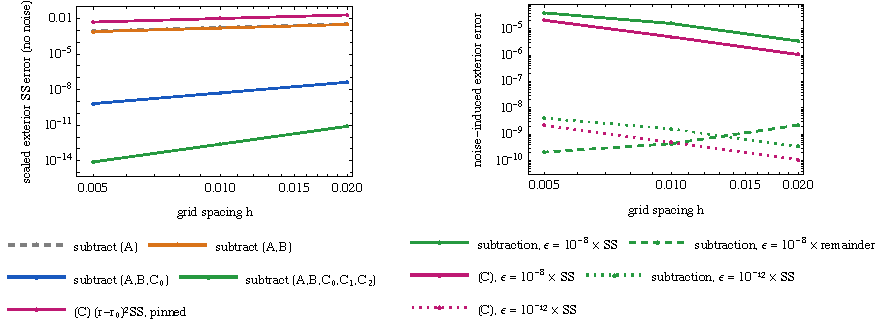
\includegraphics[width=0.85\textwidth]{fig_ss_reuse.pdf}
\caption{Continuing SS from data treated as numerical. Left: error against grid spacing for the subtraction variants and the pinned radial factor. Right: noise propagation.}
\label{fig:ssreuse}
\end{figure*}

\section{Cost of the SS quadrature}\label{app:cost}
We measured the cost of the SS piece of the exterior field for $\ell\le\ell_{\max}=10$, 20 and 30, on the real axis and on the contour.
Cost is counted as evaluations of the 3D source and as radial sample points.
Errors are maximised over $\ell$ and over exterior points, against the closed form.

\emph{Angular quadrature.}
Table~\ref{tab:angular} uses the 400-point real grid of spacing $R/200$, as in Ref.~\cite{Upton2026}, and 64 contour nodes.
The first row is the one-dimensional analogue of the adaptive quadrature of Ref.~\cite{Upton2026}.
\begin{itemize}
\item Evaluating the source once per point and projecting it onto all modes is the largest saving, a factor of 200--2000, and it applies on either axis.
\item Per point the costs are similar: 56--80 nodes in $\ln\rho$ on the real axis, against $2\times64$ or $2\times80$ on the contour.
The contour's overall advantage at $10^{-8}$, a factor of 1.2--2.8, comes from its smaller number of radial points.
\item Adaptive quadrature stops short of its own tolerance at high $\ell$.
The contour stalls at $1.6\times10^{-12}$ for $\ell_{\max}=30$, which we do not yet understand.
\end{itemize}

\begin{table}[t]
\caption{Evaluations of the 3D source for the exterior SS field to $10^{-8}$ and $10^{-12}$, $\ell_{\max}=30$.
Adaptive quadrature reaches only $7\times10^{-7}$ and $5\times10^{-10}$ (a, b); the contour stalls at $1.6\times10^{-12}$ (c).}
\label{tab:angular}
\begin{ruledtabular}
\begin{tabular}{lcc}
method & $10^{-8}$ & $10^{-12}$\\
\hline
real axis, adaptive per $(\ell,r)$ & $5.4\times10^6$\,(a) & $5.0\times10^7$\,(b)\\
real axis, shared nodes in $\ln\rho$ & $2.3\times10^4$ & $2.5\times10^4$\\
contour, rule per $\ell$ & $2.3\times10^5$ & (c)\\
contour, shared nodes & $8.2\times10^3$ & (c)\\
\end{tabular}
\end{ruledtabular}
\end{table}

\emph{Radial samples.}
On the real axis the exterior field is the Hadamard finite part of $\int G_\ell\,\mathrm{SS}_\ell\,dr$ over the worldtube.
The terms $A_\ell/\Delta r^2+B_\ell/\Delta r+C_\ell\ln|\Delta r|$ are integrated against $G_\ell$ analytically, and the remainder by quadrature.
This agrees with the contour to $2\times10^{-14}$.
Table~\ref{tab:radial} and Fig.~\ref{fig:radial} give the number of samples needed for $\ell_{\max}=30$; the counts change little with $\ell_{\max}$.
\begin{itemize}
\item Without noise, the real axis can match the contour: a grid graded toward $r_0$ needs 48--120 samples, against 64--80 contour nodes.
A uniform grid needs 100--800, provided the next two logarithmic terms, $\Delta r\ln|\Delta r|$ and $\Delta r^2\ln|\Delta r|$, are also subtracted.
\item With $10^{-8}$ relative noise on the samples, the real-axis result is $10^2$--$3\times10^5$ times less accurate than the contour's.
This noise level matches the accuracy of the numerically integrated SS source in Ref.~\cite{Upton2026}.
Subtracting $A_\ell/\Delta r^2$ amplifies the noise near $r_0$ by the same factor, so the graded grid, which samples closest to $r_0$, suffers most.
Contour samples stay at $|z-r_0|\ge0.3$ and lose only a factor of 5--8.
\end{itemize}

\begin{table}[t]
\caption{Radial source samples needed for the exterior SS field to $10^{-8}$ and $10^{-12}$, and the error when $10^{-8}$ relative noise is added to the samples (at those two configurations).
Uniform grids subtract three terms ($A$, $B$, $C_0$) or five (also $C_1\Delta r\ln|\Delta r|$ and $C_2\Delta r^2\ln|\Delta r|$); with three, 6400 samples give $1\times10^{-11}$.}
\label{tab:radial}
\begin{ruledtabular}
\begin{tabular}{lccc}
method & $10^{-8}$ & $10^{-12}$ & error with noise\\
\hline
contour & 64 & 80 & $8\times10^{-8}$, $5\times10^{-8}$\\
real, graded & 48 & 120 & $4\times10^{-4}$, $1.5\times10^{-2}$\\
real, uniform, 3 terms & 800 & $>6400$ & $9\times10^{-5}$\\
real, uniform, 5 terms & 100 & 800 & $1\times10^{-5}$, $9\times10^{-5}$\\
\end{tabular}
\end{ruledtabular}
\end{table}

\begin{figure}[t]
\centering
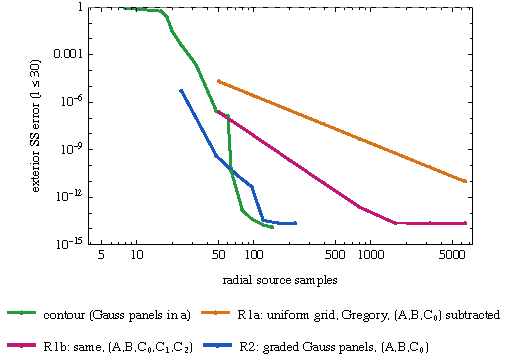
\includegraphics[width=\columnwidth]{fig_radial.pdf}
\caption{Exterior SS error ($\ell_{\max}=30$) against the number of radial source samples, without noise: contour Gauss panels, and real-axis finite-part integration on a uniform grid (with three or five subtracted terms) or on panels graded toward $r_0$.}
\label{fig:radial}
\end{figure}

\section{Convergence of the hybrid split}\label{app:convergence}
With $\PhiP=q/\rho+cq\rho^n$, the residual $\PhiR-cq\rho^n$ is $C^{n-1}$ at $\x_0$.
Its coupled-mode contributions fall as $\ell'^{-(n+3)}$, so the truncation error falls as $\ell'^{-(n+2)}_{\max}$.
The fitted slopes are $2.93$, $4.87$, $6.83$ and $8.79$ for $n=1$, 3, 5 and 7 (Fig.~\ref{fig:conv}).
With the physical boundary conditions used throughout, the error is largest next to the worldtube and decays away from it on both sides.
With Cauchy data at $r=1$ instead, any source error excites the growing solution $r^\ell$, and the error grows towards $r=10$.

Fitting the large-$\ell'$ tail with two terms of the $\Lambda_{\ell,s,n}$ functions of Refs.~\cite{Upton2026,HeffernanOttewillWardell2012} gains a factor of 18--40 at $\ell'_{\max}=20$, and up to 770 at $\ell'_{\max}=30$.
At $\ell'_{\max}=12$ the two-term fit makes the error worse; a one-term fit gains a factor of 2.5--4.3 there.
The hybrid split adds no error of its own: the Cauchy step of the contour solve contributes below $2\times10^{-16}$, less than $10^{-11}$ of the total, and the split error equals the mode-truncation error.

\begin{figure*}[t]
\centering
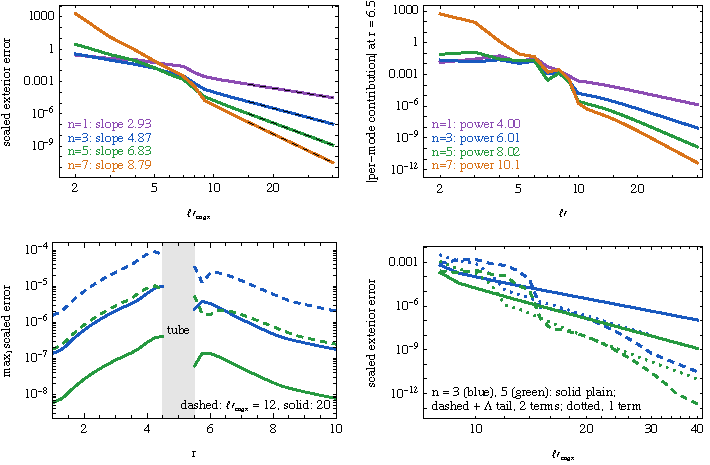
\includegraphics[width=0.85\textwidth]{fig_hybrid_convergence.pdf}
\caption{Hybrid split, $Q=\tfrac12\partial_z^2(AB)$, $k=0$.
Top: error against $\ell'_{\max}$ with fitted slopes, and per-mode contributions against $\ell'$.
Bottom left: error against $r$.
Bottom right: tail acceleration.}
\label{fig:conv}
\end{figure*}

\section{Comparison with Musaeus, Pound and Upton}\label{app:mpu}
\emph{Mode-level finite part.}
For the operator $r^2\partial_r^2-2r\partial_r-(\ell-1)(\ell+2)$ with the Green's function of their Eq.~140, and sources $A/\Delta r^4+B/\Delta r^3+C/\Delta r^2+D/\Delta r$, we compared three calculations for $\ell=2$--$6$:
\begin{itemize}
\item their prescription (Eqs.~141 and A2--A5);
\item an independent Taylor-subtracted finite part, which agrees with it to below $10^{-38}$, independently of the cutoff;
\item the contour integral $\Re\int_CG\,S\,dz$, which agrees with both to $4\times10^{-34}$ for five choices of worldtube radius and contour height.
\end{itemize}
Their closed form, Eq.~142, is confirmed.

\emph{$T_Q$ and the mode-level $\delta$ content} (exact puncture, $Q=\tfrac12\partial_z^2(AB)$).
The canonical SR is $q\,\partial_z^2(\PhiR/\rho)$, a derivative of an integrable function.
Its 4D finite part is the ball-excluded principal value, and the difference between the two is $T_Q=-\tfrac{4\pi}{3}q\PhiR(\x_0)\delta^3$, verified to $10^{-21}$.
At mode level, the total $\delta$ coefficient is $c_\ell=-4\pi q\PhiR(\x_0)Y_{\ell0}(0)/r_0^2$, which splits as $\tfrac23c_\ell$ from the finite part plus $\tfrac13c_\ell$ from $T_Q$.
Scaled exterior errors for each prescription are listed in Table~\ref{tab:tq}.
The shell (mode-level) and ball (4D) regulators do not commute for the trace-free $\rho^{-3}$ term: a term proportional to $B'/(B+B')$ survives.

\begin{table}[t]
\caption{Scaled exterior errors ($\ell\le6$) for different treatments of the SR source.}
\label{tab:tq}
\begin{ruledtabular}
\begin{tabular}{lc}
prescription & error\\
\hline
contour, canonical source & $<10^{-29}$\\
4D finite-part modes $+\;T_Q$ (their Eq.~24) & $<10^{-19}$\\
4D finite-part modes, without $T_Q$ & $0.18$--$1.1$\\
pointwise modes, their Eq.~105 $+\;T_Q$ & $0.37$--$2.2$\\
pointwise modes, no $\delta$ terms & $0.55$--$3.3$\\
\end{tabular}
\end{ruledtabular}
\end{table}

\section{Numerical details}\label{app:numerics}
All computations use working precision 30 and exact rational parameters.
Radial solves use the boundary conditions $\psi'=\ell\psi/r$ at $r=1$ and $\psi'=-(\ell+1)\psi/r$ at $r=10$; for a source on $[1,10]$ these make the free-space Green's function $-r^{\prime2}r_<^\ell/[(2\ell+1)r_>^{\ell+1}]$ exact, and the exact reference is adjusted to the same conditions.
NDSolve is run with PrecisionGoal 20, AccuracyGoal 35 and \texttt{InterpolationOrder -> All}.
Contour sources are evaluated at numerical $y(a)$: symbolic composition expands them into high-degree polynomials and loses all accuracy.
The Cauchy step uses Gauss quadrature after subtracting the cubic Taylor polynomial of $s$ about $\Re z$, which is integrated analytically; the source on the contour is represented piecewise at 40-digit precision.
The implementation is checked by more than 2,000 automated tests.

\begin{thebibliography}{99}
\bibitem{Warburton2021}
N.~Warburton, A.~Pound, B.~Wardell, J.~Miller, and L.~Durkan,
Phys.\ Rev.\ Lett.\ \textbf{127}, 151102 (2021).

\bibitem{Wardell2023}
B.~Wardell, A.~Pound, N.~Warburton, J.~Miller, L.~Durkan, and A.~Le~Tiec,
Phys.\ Rev.\ Lett.\ \textbf{130}, 241402 (2023).

\bibitem{Pound2020}
A.~Pound, B.~Wardell, N.~Warburton, and J.~Miller,
Phys.\ Rev.\ Lett.\ \textbf{124}, 021101 (2020).

\bibitem{BarackPound2019}
L.~Barack and A.~Pound,
Rep.\ Prog.\ Phys.\ \textbf{82}, 016904 (2019).

\bibitem{MusaeusPoundUpton2026}
J.~Musaeus, A.~Pound, and S.~D.~Upton,
arXiv:2609.10521 [gr-qc] (2026).

\bibitem{MillerWardellPound2016}
J.~Miller, B.~Wardell, and A.~Pound,
Phys.\ Rev.\ D \textbf{94}, 104018 (2016).

\bibitem{Upton2026}
S.~D.~Upton, B.~Wardell, A.~Pound, N.~Warburton, and L.~Barack,
arXiv:2508.00087 [gr-qc] (2026).

\bibitem{BarackGolbourn2007}
L.~Barack and D.~A.~Golbourn,
Phys.\ Rev.\ D \textbf{76}, 044020 (2007).

\bibitem{VegaDetweiler2008}
I.~Vega and S.~Detweiler,
Phys.\ Rev.\ D \textbf{77}, 084008 (2008).

\bibitem{GelfandShilov}
I.~M.~Gel'fand and G.~E.~Shilov,
\emph{Generalized Functions}, Vol.~1 (Academic Press, New York, 1964).

\bibitem{HeffernanOttewillWardell2012}
A.~Heffernan, A.~Ottewill, and B.~Wardell,
Phys.\ Rev.\ D \textbf{86}, 104023 (2012).

\end{thebibliography}

\end{document}
